\documentclass{llncs}

%\usepackage{makeidx}  % allows for indexgeneration
\usepackage{graphicx}
\usepackage{listings}
\usepackage{color}

%some utils macros
\definecolor{listinggray}{gray}{0.97}
\lstset{
	basicstyle=\scriptsize,
	basewidth=0.50em,
	backgroundcolor=\color{listinggray},
	keywordstyle=\bfseries,
	stringstyle=\itshape,
	commentstyle=\itshape,
	%basicstyle=\small\tt,
	showspaces=false,
	showtabs=false,
	showstringspaces=false,
	frame=trbl,
	extendedchars=true,
	numbers=none,
	aboveskip=0cm,
	belowskip=0cm,
	xleftmargin=0cm,
	xrightmargin=0cm
}
\lstdefinelanguage{RDF}[]{XML}{%
	morekeywords = {rdf:RDF, rdf:about, rdf:resource, rdf:Description,
			sioc:Post, sioc:id, sioc:has_creator, sioc:content, 
			sioc:has_reply, dc:title, dcterms:created,
			swaml:previousByDate, swaml:nextByDate }
}
\lstdefinelanguage{SPARQL}{%
	morekeywords = {PREFIX, SELECT, DISTINCT, WHERE, FROM }
}

\begin{document}

\title{Mailing lists meet the Semantic Web}

\titlerunning{Mailing lists meet the Semantic Web}

\author{
Sergio Fern\'andez\inst{1} 
\and
Diego Berrueta\inst{1} 
\and
Jose E. Labra\inst{2}
}

\authorrunning{Sergio Fern\'andez et al.}

\tocauthor{Sergio Fern\'andez, Diego Berrueta, Jose E. Labra} 

\institute{%
Fundaci\'on CTIC, \\
Gij\'on, Asturias, Spain,\\
\email{\{sergio.fernandez,diego.berrueta\}@fundacionctic.org}
\and
Universidad de Oviedo,\\
Computer Science Department,\\
Oviedo, Asturias, Spain,\\
\email{labra@uniovi.es}\\
}

\date{18 February 2007}

\maketitle

\begin{abstract}

Mailing list archives (i.e., the compilation of the messages posted up-to-now) are often 
published on the web and indexed by conventional search engines. They 
store a vast knowledge capital. However, the ability to automatically 
recognize and process the information is mostly lost at publishing time. 
As a result, the current mailing list archives are difficult to query and have 
a limited use. This paper describes an usage of the Semantic Web technologies 
in order to avoid the information loss and to allow new applications 
to exploit the information in a more powerful way.

\end{abstract}

\section{Introduction}

Electronic mail (e-mail) remains one of the most
popular applications of the Internet. Besides direct messaging
between individuals, mailing lists exist as private or public
forums for information exchange in communities with shared interests.
Mailing list archives are compilations of the previously posted
messages that are often converted into static HTML pages for their
publication on the web. They represent a noteworthy portion of
the contents that are indexed by web search engines, and they
capture an impressive body of knowledge that, however, is difficult
to locate and browse.

The root of these problems can be traced back to the translation
procedure that is run to transform the e-mail messages into static
HTML pages. This task is fulfilled by scripts that create an
static HTML page for each message in the archive. In addition,
some indexes (by date, by author, by thread) are generated and
usually splitted by date ranges to avoid excessive growth.
On the one hand, this 
fixed structure reduces the flexibility when users browse the
mailing list archives using their web browsers. On the other hand, some 
of the meta-data that were associated to each e-mail message are lost
when the message is rendered as HTML for presentational purposes.

We propose to use an ontology and RDF (Resource Description
Framework~\cite{RDF}) to publish the mailing list archives into 
the (Semantic) web, while retaining the meta-data that were present in 
the messages. Additionally, by doing so, the information could be
merged and linked to other vocabularies, such as FOAF.

The rest of the paper is organized as follows: 
Section~\ref{sec:SIOC} introduces the SIOC ontology and our extensions 
to it, and then some software applications are described in 
Section~\ref{sec:tools}. We close the paper with the conclusions and 
a discussion on future plans in Section~\ref{sec:conclusions}.

\section{\label{sec:SIOC}SIOC}

An ontology to capture the meta-data of a discussion forum, such as
a mailing list, was clearly recognized as the first milestone to
fulfill the purpose of the project. Fortunately, DERI Galway has 
developed SIOC (Semantically-Interlinked Online
Communities\footnote{\url{http://sioc-project.org/}}), an ontology that provides a vocabulary to interconnect 
different discussion methods such as blogs, web-based forums and mailing 
lists~\cite{Breslin2006,Breslin2005}. Indeed, SIOC has a wider 
scope than just mailing lists, and groups all kinds of online discussion 
primitives in a generic \textsf{sioc:Forum} concept. Each forum represents 
an online community of people that share a common interest. The goal 
of SIOC is to interconnect these online communities. Other relevant concepts 
of the ontology are \textsf{sioc:User} and \textsf{sioc:Post}, which 
model respectively the members of the communities and the content they 
produce.

\begin{figure}[ht]
 \centering
 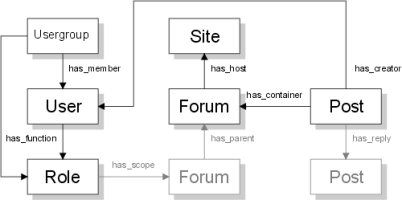
\includegraphics[width=7cm]{images/sioc-terms.png}
 \caption{SIOC ontology terms}
\end{figure}

The SIOC ontology was designed to express the information contained
both explicitly  and implicitly in Internet discussion methods. Several 
software applications, usually deployed as plug-ins, are already available 
to export SIOC data from some popular blogging platforms and content 
management systems. The effort, however, is focused on web-based communities 
(weblogs, webforums), while little has been done so far to extend the coverage 
to legacy non-web communities, such as mailing lists and Usenet groups.

SIOC is specified in OWL, and their instances can be expressed
in RDF. Therefore, they can be easily linked to other ontologies.
The obvious choice here is FOAF~\cite{FOAF}, which provides
powerful means to describe the personal data of the members of
a community.

\subsection{Extending SIOC Ontology}

SIOC was quickly identified as an almost perfect match for our
purpose. Each mailing list becomes an instance of \textsf{sioc:Forum},
messages sent to the list become instances of \textsf{sioc:Post}
(as well as their replies), and the people subscribed to the
list are \textsf{sioc:User}s. The Dublin Core~\cite{DublinCore}
vocabulary is used to capture meta-data such as the message
date or title.

However, additional object properties were required
in order to retain the sequence of messages published in a
mailing list. Thus, we extended the SIOC ontology with two
properties\footnote{These properties are defined in a separate
namespace, \url{http://swaml.berlios.de/ns/0.2\#}}:
\textsf{swaml:previousByDate} and \textsf{swaml:nextByDate}. Both properties
are defined with \textsf{sioc:Post} as their domain and range.
An RDF representation of a sample message is shown in
Figure~\ref{fig:rdfexample}.

\begin{figure}[ht]
\lstset{language=RDF}
\begin{lstlisting}
<rdf:RDF
  xmlns:dcterms='http://purl.org/dc/terms/'
  xmlns:sioc='http://rdfs.org/sioc/ns#'
  xmlns:rdf='http://www.w3.org/1999/02/22-rdf-syntax-ns#'
  xmlns:swaml='http://swaml.berlios.de/ns/0.2#'
  xmlns:dc='http://purl.org/dc/elements/1.1/'
  xml:base='http://swaml.berlios.de/demo/'>
  <sioc:Post rdf:about="2006-Oct/post-50.rdf">
    <dc:title>SIOC properties cardinality</dc:title>
    <sioc:has_creator rdf:resource="subscribers.rdf#s4"/>
    <dcterms:created>Thu, 12 Oct 2006 23:59:26 +0200</dcterms:created>
    <sioc:content><!-- ommitted --></sioc:content>
    <sioc:has_reply rdf:resource="2006-Oct/post-51.rdf"/>
    <swaml:previousByDate rdf:resource="2006-Oct/post-49.rdf"/>
    <swaml:nextByDate rdf:resource="2006-Oct/post-51.rdf"/>
  </sioc:Post>
</rdf:RDF>
\end{lstlisting}
\caption{SIOC Post example in RDF/XML}
\label{fig:rdfexample}
\end{figure}

\section{\label{sec:tools}Software tools}

The ontology itself provides no service to end users. Software tools
are required, and we built two of them as part of this
project\footnote{Our applications are available at \url{http://swaml.berlios.de/}}.

\begin{itemize}
  \item SWAML is a non-interactive, command-line application whose main
	purpose is to translate mailboxes into \textsf{sioc:Forum}
        instances in RDF.
  \item Buxon is a graphical browser for \textsf{sioc:Forum} instances.
\end{itemize}

\begin{figure}[ht]
 \centering
 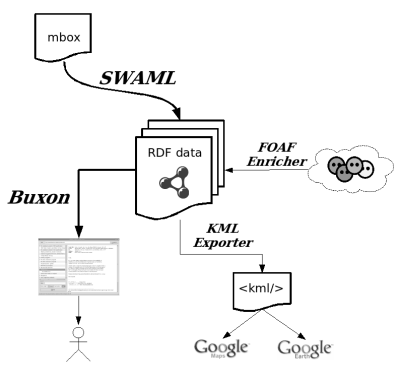
\includegraphics[width=9cm]{images/swaml.png}
 \caption{\label{fig:swaml-and-buxon}Buxon is an end-user application
that consumes
\textsf{sioc:Forum} instances, which in turn can be generated from mailboxes
using SWAML.}
\end{figure}

Each tool has a precisely defined role, fulfilling the need to
generate RDF data and to consume data, respectively, as depicted
in Figure~\ref{fig:swaml-and-buxon}. The following paragraphs
provide further detail on SWAML and Buxon.

\subsection{SWAML}

SWAML covers the data-generation phase, and it is intended to be
used by mailing list administrators, who usually have access to
the archives in raw format. The most popular format for
mailing list archives is the ``mailbox'' (or ``mbox''), as defined
in RFC~4155~\cite{RFC4155}. SWAML is essentially a mailbox parser
implemented in Python. Its output is a number of SIOC instances
(\textsf{Forum}, \textsf{Post}s and \textsf{User}s) in a set
of RDF files. SWAML is a highly configurable, non-interactive
application designed to be invoked by the system task scheduler.

Parsing the mailbox and rebuilding the discussion threads may be
sometimes tricky. Although each mail message has a supposedly unique
identifier in its header (\textsf{Message-ID}, defined by
RFC~2822~\cite{RFC2822}), in practice its uniqueness cannot be
taken for granted. Actually, we have found some
messages with repeated identifiers in some mailing lists,
probably due to non-RFC compliant mail transport agents.
Therefore, SWAML assumes that any reference to a message
(such those created by the \textsf{In-Reply-To} header)
is in fact a reference to the most recent message with that ID
in the mailbox (obviously, only previous messages are
considered). SWAML builds a tree for in-memory representation
of the conversation threads, so \textsf{sioc:Post}s can be
properly linked.

Actually, SWAML goes further than just a format-translation
tool. A dedicated subrutine that runs a part of the batch
execution, but may be also separately invoked on any
\textsf{sioc:Forum}, tries to find a FOAF description for
each \textsf{sioc:User}. To the best of our knowledge, there is not
any web service to fetch FOAF descriptions from a given e-mail
address, so we mocked it. Some of the authors of this paper are also
currently working
on a functional implementation of such a service as part of a
different project.

The last step of the SWAML processing chain generates a
KML~\cite{Ricket2006} file that contains the geographical coordinates of
the mailing list subscribers. The information is fetched from their
FOAF descriptions, therefore it is only available for those
subscribers whose FOAF description contains the coordinates
using the basic \textsf{geo} vocabulary by Dan
Brickley~\cite{Brickley2006}.
Figure~\ref{fig:googlemaps} depicts a graphical representation
of the KML file for a sample mailing list.

\begin{figure}[ht]
 \centering
 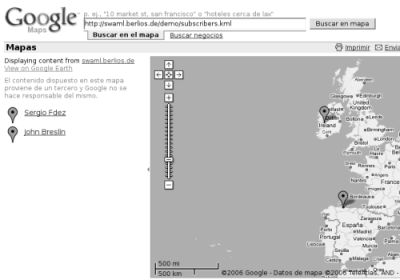
\includegraphics[width=9cm]{images/googlemaps.png}
 \caption{\label{fig:googlemaps}Plotting the geographical coordinates of
the members of a mailing list using Google Maps.}
\end{figure}

\subsection{Buxon}

Buxon is a multi-platform desktop application written in PyGTK.
It allows end users to browse the archives of mailing lists as if
they were using their desktop mail application. Buxon takes
the URI of a \textsf{sioc:Forum} instance (for example, a mailing list
exported by SWAML, although any \textsf{sioc:Forum} instance
is valid) and fetches the data, retrieving additional files
if necessary. Then, it rebuilds the conversation structure and
displays the familiar message thread list (see Figure~\ref{fig:buxon}).

\begin{figure}[ht]
 \centering
 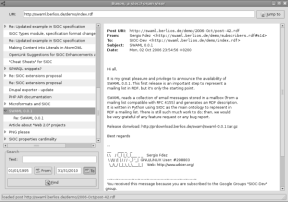
\includegraphics[width=9cm]{images/buxon.png}
 \caption{\label{fig:buxon}Buxon browsing SIOC-Dev mailing list}
 %FIXME: add a screenshot of v0.0.4
\end{figure}

Buxon also gives users the ability to query the messages, searching
for terms or filtering the messages in a date range. All these queries
are internally translated to SPARQL~\cite{SPARQLProtocol} to be executed
over the RDF graph. Newer versions of Buxon can, at user's request, send 
the \textsf{sioc:Forum} URI to PingTheSemanticWeb.com\footnote{\url{http://pingthesemanticweb.com/}}, 
a social web service that tracks semantic web documents. That way, Buxon
contributes to establish an infrastructure that lets people easily create, 
find and publish RDF documents.

\begin{figure}[ht]
\lstset{language=SPARQL}
\begin{lstlisting}
PREFIX sioc: <http://rdfs.org/sioc/ns#>
PREFIX rdf: <http://www.w3.org/1999/02/22-rdf-syntax-ns#>
SELECT ?title
FROM <http://swaml.berlios.de/demo/index.rdf>
WHERE
{
  ?x rdf:type sioc:Forum .
  ?x sioc:container_of ?message .
  ?message sioc:has_creator ?creator .
  ?creator sioc:name "Diego Berrueta" .
  ?message dc:title ?title
}
\end{lstlisting}
\caption{SPARQL query to extract all the posts sent to any \textsf{sioc:Forum} instance.}
\label{fig:sparqlquery}
\end{figure}

\section{\label{sec:conclusions}Conclusions and Future Work}

There is a lot of ongoing effort to translate data already reachable
on the web into formats which are Semantic Web-friendly. Most of that 
work focuses on relational databases, micro-formats and web services. 
However, at the time of this writing and to the best of our knowledge, 
e-mail was almost excluded from the Semantic Web. This project, in 
combination with the generic SIOC framework, fills this gap, conveniently 
providing an ontology and a parser to publish machine-readable versions 
of the archives of the countless mailing lists.

The SWAML project fulfills a much-needed requirement for the Semantic Web: 
to be able to refer to semantic versions of email messages and their 
properties using a resource URI. By reusing the SIOC vocabulary for describing
online discussions, SWAML allows users of SIOC to refer to email messages 
from other discussions taking place on forums, blogs, etc., so that distributed 
conversations can occur across these discussion media. Also, by providing email 
messages in SIOC format, SWAML are providing a rich source of data, namely 
mailing lists, for use in SIOC applications.

Some benefits arouse from the availability of these data. In the first
place, data can be fetched by user applications to provide handy browsing
through the archives of the mailing lists, providing features that
exceed what is now offered by static HTML versions of the archives on
the web.

Secondly, the bot crawlers of the web search engines can use the enhanced
expressivity of the RDF data to refine search results. For instance, it
becomes possible to filter out repeated messages, advance in the fight against
spam, or introduce additional filter criteria in the search forms.

Another consequence of no lesser importance is that each e-mail message
is assigned a URI that can be resolved to a machine-readable description
of the message. This actually makes possible to link a message like
any other web resource, and therefore enriches the expressivity of the
web.

We are exploring some directions for future work. Some of them are:

\begin{itemize}
  \item Integration of the SWAML process with a popular HTML-based
        mailing list archiver, such as Hypermail or Pipermail, would be
        a giant push to speed up the adoption of SWAML. It is well
        known that one of the most awkward problems of any technology
        is to gain a critical mass of users. The semantic web is not
        an exception. A good recipe to tackle this problem is to
        integrate the new technologies into old tools, making
        a smooth transition without requiring any extra effort from
        the users. Merging the SWAML process into the batch flow of
        tools such as Hypermail would allow to generate both
        HTML and RDF versions of the archive. Those could reside
        side-by-side on the web server, even sharing the same URI
        by means of content-negotiation~\cite{Recipes}.
  \item Actually, integration could be pushed further away through
        RDFa~\cite{Birbeck2006}, embedding the RDF content into the
        XHTML documents.
  \item So far, no semantic annotation relative to the meaning of
        the messages is considered. Obviously, such information can not
        be derived from a RFC 4155-compliant mailbox.
        However, it is
        conceivable that it can be added by other means, for instance,
        by social tagging using folksonomies, or by parsing the RDFa
        that can exist in the messages that are send in XHTML format.
        The inherent community-based nature of mailing lists may
        be exploited to build recommendation systems~\cite{Celma2006}.
  \item The meta-data extracted from a mailing list archive can be
        quite huge. Even after removing the body of the messages, the
        XML/RDF meta-data of a mailing list containing 1000 messages may
        have a size of 4 MBytes, with a linear growth. It is not uncommon
        for a busy mailing list to generate this volume of messages
        monthly. Hence, it is imperative to design a mechanism to
        fragmentate the dataset. The SWAML process splits each message
        in a separate RDF document, but this arbitrary decision clearly
        does not fit every application. A much better solution would be to
        create an easy-to-deploy SPARQL endpoint~\cite{SPARQLProtocol},
        that translates the
        decision on how to partition the data to the final
        application~\cite{Pan2006}.
  \item It is not always possible to obtain a mailbox file for a mailing
        list. For these cases, an alternative is envisaged: a high-capacity
        GMail account can be subscribed to the mailing list with the unique
        purpose of collecting and storing the messages. A simple extension
        to SWAML that makes possible to import the contents of a GMail
        account has been developed.

\end{itemize}

\section*{Acknowledgements}

The authors would like to express their gratitude to Dr. John Breslin and
Uldis Bojars from DERI Galway, whose support and contributions have been of 
great help to this project.

\bibliographystyle{abbrv}
\bibliography{../references}
%
\end{document}
